% ====================================================================
% VİZE RAPOR ŞABLONU – Türk Masalları Derlemesi Web Sayfası
% --------------------------------------------------------------------
% DERLEME: Overleaf'te Menu > Compiler > XeLaTeX (pdfLaTeX de çalışır).
%
% KURALLAR (şablonu kullanmadan önce okuyun):
%  1. Bölüm başlıklarını SİLMEYİN ve sırasını DEĞİŞTİRMEYİN.
%  2. [KÖŞELİ PARANTEZ] içindeki ve gri renkli açıklama metinlerini
%     kendi bilgilerinizle değiştirin; açıklama metinlerini silin.
%  3. MEBİS'e YALNIZCA bu raporun PDF'ini yükleyin.
%     ZIP ve HTML dosyası YÜKLEMEYİN. Tüm kontroller GitHub'dan yapılır.
%  4. Kapaktaki GitHub ve YouTube bağlantıları doğru ve tıklanabilir
%     olmalıdır. Teslimden önce PDF'teki bağlantılara tıklayıp deneyin.
%  5. Haftalık katkı tablosundaki görseller için resim dosyalarını
%     (hafta1.png, hafta2.png, ...) Overleaf projesine yükleyin.
%     Dosya adlarında boşluk ve Türkçe karakter kullanmayın.
%     Resim yoksa tabloda "görsel ekleyin" kutusu görünür.
%  6. Yapay zekâ kullandıysanız Bölüm 5'i doldurun.
% ====================================================================
\documentclass[12pt,a4paper]{article}

\usepackage{iftex}
\ifPDFTeX
  \usepackage[T1]{fontenc}
  \usepackage[utf8]{inputenc}
\else
  \usepackage{fontspec}
\fi
\IfFileExists{turkish.ldf}{\usepackage[turkish]{babel}}{\usepackage[provide=*,turkish]{babel}}
\usepackage[margin=2.4cm]{geometry}
\usepackage{setspace}
\usepackage{graphicx}
\usepackage{booktabs}
\usepackage{longtable}
\usepackage{array}
\newcolumntype{P}[1]{>{\raggedright\arraybackslash}p{#1}}
\usepackage{colortbl}
\usepackage{xcolor}
\usepackage{enumitem}
\usepackage{listings}
\usepackage{amssymb}
\usepackage{caption}
\usepackage{fancyhdr}
\usepackage{hyperref}

\setlength{\headheight}{15pt}
\setlength{\emergencystretch}{3em}
\onehalfspacing
\setlength{\parindent}{0pt}
\setlength{\parskip}{6pt}
\setlist{itemsep=2pt, topsep=4pt}
\hypersetup{colorlinks=true, linkcolor=blue!50!black, urlcolor=blue!50!black}

\definecolor{ana}{HTML}{14325C}
\definecolor{acik}{HTML}{EEF2F8}

\lstset{basicstyle=\ttfamily\small, backgroundcolor=\color{acik},
  frame=single, rulecolor=\color{ana}, breaklines=true,
  columns=fullflexible, keepspaces=true, showstringspaces=false}

\pagestyle{fancy}
\fancyhf{}
\fancyhead[L]{Masalsı Pırıltı}
\fancyhead[R]{Vize Raporu}
\fancyfoot[C]{\thepage}

% ---------- Yardımcı komutlar ----------
% Gri açıklama metni (silinecek yönergeler için)
\newcommand{\aciklama}[1]{{\color{gray}\itshape (#1)}}

% Haftalık tablo görseli: dosya yoksa "görsel ekleyin" kutusu çıkar
\newcommand{\haftagorsel}[1]{%
  \IfFileExists{#1}{%
    \includegraphics[width=\linewidth,height=4.2cm,keepaspectratio]{#1}%
  }{%
    \fbox{\parbox[c][2.6cm][c]{\dimexpr\linewidth-2\fboxsep-2\fboxrule\relax}{%
      \centering\small\color{gray} Ekran görüntüsü / görsel ekleyin\\ \texttt{#1}}}%
  }%
}
% Haftalık katılım kutuları (işaretlemek için $\square$ yerine $\boxtimes$ yazın)
\newcommand{\katilimkutulari}{\par\vspace{3pt}\small $\square$ Ders içinde katılım sergiledim\par $\boxtimes$ Telafi yaptım}

% Ek görsel: dosya yoksa hiçbir şey göstermez
\newcommand{\haftaek}[1]{%
  \IfFileExists{#1}{\\[4pt]\includegraphics[width=\linewidth,height=4.2cm,keepaspectratio]{#1}}{}%
}

% ---------- Kapak bilgileri ----------
\newcommand{\universite} {İSTANBUL MEDİPOL ÜNİVERSİTESİ / GÖRSEL
İLETİŞİM TASARIMI  }  
\newcommand{\dersadi}{PROGRAMLAMAYA GİRİŞ}
\newcommand{\hocaadi}{MERAL ŞENTÜRK}
\newcommand{\ogrenciadi}{İREM AKPINAR}
\newcommand{\ogrencino}{86240029}
\newcommand{\projeadi}{Masalsı Pırıltı}
% Bağlantıları tam adres olarak yazın (https:// ile başlayarak)
\newcommand{\githublink}{\url{https://github.com/KULLANICI-ADI/DEPO-ADI}}
\newcommand{\youtubelink}{\url{https://www.youtube.com/watch?v=VIDEO-KIMLIGI}}

\begin{document}

% ====================================================================
% KAPAK
% ====================================================================
\hypersetup{pageanchor=false}
\begin{titlepage}
\centering
\vspace*{1cm}
{\large \universite \par}
\vspace{1.8cm}
{\Huge\bfseries\color{ana} \projeadi \par}
\vspace{0.4cm}
{\Large Türk Masalları Derlemesi Web Sayfası \par}
{\large Vize Raporu \par}
\vspace{1.8cm}
{\large \textbf{Ders:} \dersadi \par}
{\large \textbf{Öğretim Üyesi:} \hocaadi \par}
\vspace{1.2cm}
{\large \textbf{Hazırlayan:} \ogrenciadi \par}
{\large \textbf{Öğrenci No:} \ogrencino \par}
\vspace{1.8cm}
\fbox{\parbox{0.88\linewidth}{\centering\vspace{6pt}
{\large\bfseries Proje Bağlantıları}\\[8pt]
\textbf{GitHub deposu:}\\ \githublink \\[8pt]
\textbf{YouTube sunum videosu:}\\ \youtubelink
\vspace{6pt}}}
\vfill
{\large \today \par}
\end{titlepage}
\hypersetup{pageanchor=true}

\tableofcontents
\newpage

% ====================================================================
\section{Giriş}
% ====================================================================
\aciklama{Projenin amacını, neyi neden yaptığınızı ve raporun içeriğini 5--8 cümleyle
anlatın. Ödev gereksinimlerini (8--12 masal, tek HTML dosyası, içsel CSS ve içsel
JavaScript) nasıl karşıladığınızı belirtin.}

\subsection{Proje Özeti}
Masalsı pırıltı,sekiz masalı illüstrasyonlarla bir araya getiren etkileşimli bir masal okuma web sitesidir.Projenin amacı,ziyaretçilere masalsı bir atmosfer içinde kolay ve rahat bir okuma deneyimi sunmaktır.Sitede masal adına göre arama,temaya göre filtreleme,rastgele bir masal seçme, masalı okurken isteğe göre yazı boyutunu değiştirme ve gece moduna geçme gibi özellikler bulunmaktadır.Tasarımda renk paleti olarak lacivert,mor ve turkuaz tonları seçilmiştir.Ayrıca sitenin masalsı atmosferini yansıtmak amacıyla küçük hareketli ışıklar kullanılmıştır.

\subsection{Gereksinimlerin Karşılanması}
\begin{center}
\rowcolors{2}{acik}{white}
\begin{tabular}{@{}p{8.2cm}c@{}}
\toprule
\rowcolor{ana}\textcolor{white}{\textbf{Gereksinim}} & \textcolor{white}{\textbf{Durum}} \\
\midrule
Masal sayısı 8--12 arasında (8 masal)         & $\boxtimes$ \\
Tek HTML dosyası                                    & $\boxtimes$ \\
Stil kodları içsel (\texttt{<style>} içinde)        & $\boxtimes$ \\
Betik kodları içsel (\texttt{<script>} içinde)      & $\boxtimes$ \\
İnternetsiz açılıp çalışıyor                        & $\boxtimes$ \\
JavaScript sayfada anlamlı bir işlev görüyor        & $\boxtimes$ \\
Masal metinleri kendi cümlelerimle yazıldı          & $\boxtimes$ \\
Sayfa telefonda da düzgün görünüyor                 & $\boxtimes$ \\
\bottomrule
\end{tabular}
\end{center}
\aciklama{Karşıladığınız her satırın kutusunu $\boxtimes$ ile değiştirin.}

% ====================================================================
\section{Masalların Seçimi}
% ====================================================================
\aciklama{Hangi masalları, hangi ölçütlere göre seçtiniz? Tabloyu masal sayınıza göre
düzenleyin (en az 8, en fazla 12 satır). Kullandığınız kaynakları Kaynakça'ya yazın.}

\begin{longtable}{@{}cP{4cm}P{3cm}P{5.4cm}@{}}
\toprule
\textbf{No} & \textbf{Masal} & \textbf{Tür} & \textbf{Seçilme nedeni} \\
\midrule
\endhead
1 & Kurnaz Kurt & Hayvan Masalı & Kurnazlık teması \\
2 & Sihirli Tavşan & Olağanüstü masal & Sihirli bir macera. \\
3 & Altın Saçlı Kız & Olağanüstü masal & Açgözlülüğün zararını göstermesi. \\
4 & Limon Kız & Olağanüstü masal & Olağanüstü olaylarıyla merak uyandırdı.\\
5 & Akıllı Ormancı & Hayvan masalı &  Aklın güçten üstünlüğünü işlemesi.  \\
6 & Altın Bülbül & Olağanüstü masal & Macera ve merak duygusu uyandırdı. \\
7 & Zümrüdüanka Kuşu & Fantastik Anlatı & Umut ve İyiliği konu alması.\\
8 & Gülen Ayva Ağlayan Nar & Fantastik Anlatı & Cesaret ve empatiyi konu alması. \\
\bottomrule
\end{longtable}

% ====================================================================
\section{Tasarım Kararları}
% ====================================================================
\aciklama{Masal temasını yansıtmak için orman, gece ve ışık
unsurlarının yer aldığı bir görsel dil tercih ettim.
Her masalın içeriğine uygun illüstrasyonlar kullanıldı.
Küçük hareketli ışık noktaları, Masalsı Pırıltı adını
desteklerken ziyaretçiyi masalları keşfetmeye yönlendiriyor.
Kitap ve pırıltı simgelerini birleştiren logo da sitenin
okuma amacını yansıtıyor.}

\subsection{Konuya Uygunluk}
Türk masallarındaki orman, saray ve olağanüstü varlıklardan
yola çıkarak masalsı bir atmosfer oluşturdum. Lacivert ve
mor tonlarını geceyi ve gizemi, turkuaz rengini ise ışıkları ve sihirli olayları çağrıştırması için seçtim. Başlıklarda kullanılan Georgia yazı tipi, basılı masal kitaplarını hatırlatıyor. İllüstrasyonlar ise her masalın karakterlerini ve geçtiği ortamı yansıtarak okuyucunun hikâyeyi hayal etmesini kolaylaştırıyor.

\subsection{Renk Paleti ve Yazı Tipi}
\begin{center}
\rowcolors{2}{acik}{white}
\begin{tabular}{@{}llP{6.4cm}@{}}
\toprule
\rowcolor{ana}\textcolor{white}{\textbf{Ad}} & \textcolor{white}{\textbf{Kod}} & \textcolor{white}{\textbf{Nerede / neden kullandınız?}} \\
\midrule
Lacivert & \texttt{\#0B1630} & Gece atmosferi için arka planda. \\
Mor & \texttt{\#B7A0E6} & Masalsı etki ve vurgu için. \\
Krem & \texttt{\#FFFAF2} & Okuma alanının zemininde. \\
Georgia / Arial & -- & Başlıklarda masalsı görünüm, arayüzde kolay okunabilirlik için. \\
\bottomrule
\end{tabular}
\end{center}

\subsection{Okunabilirlik, Gezinme ve Duyarlı Tasarım}
\begin{itemize}
  \item \textbf{Okunabilirlik:} Yazı boyutu değiştirilebilir. Satır uzunluğu sınırlandırıldı,
satır aralıkları ferah tutuldu. Krem zemin üzerinde koyu
metin kullanılarak okuma kolaylaştırıldı.
  \item \textbf{Gezinme:} Kullanıcı masallara kartlardan, arama kutusundan veya tema
filtrelerinden ulaşabilir. Rastgele masal seçeneği de bulunur.
  \item \textbf{Duyarlı tasarım:} Ekran daraldığında masal kartları daha az sütunda gösterilir.
Menü, yazılar ve okuma alanı ekran genişliğine göre düzenlenir.
  \item \textbf{Tutarlılık:} Sayfa boyunca aynı renk paleti, yazı tipleri, buton biçimleri
ve benzer boşluklar kullanılarak görsel bütünlük sağlandı.
\end{itemize}

\subsection{Ekran Görüntüleri}

\begin{center}
  \haftagorsel{ekran-mobil.png}

  \small Sayfanın telefon görünümü
\end{center}

\begin{center}
  \haftagorsel{ekran-masaustu.png}

  \small Sayfanın bilgisayar görünümü
\end{center}

\begin{center}
  \haftagorsel{okuma ekranı.png}

  \small Masal okuma ekranı
\end{center}

\begin{center}
  \haftagorsel{Masal kartları.png}

  \small Masal kartlarının görünümü
\end{center}

% \begin{figure}[h]
%   \centering
%   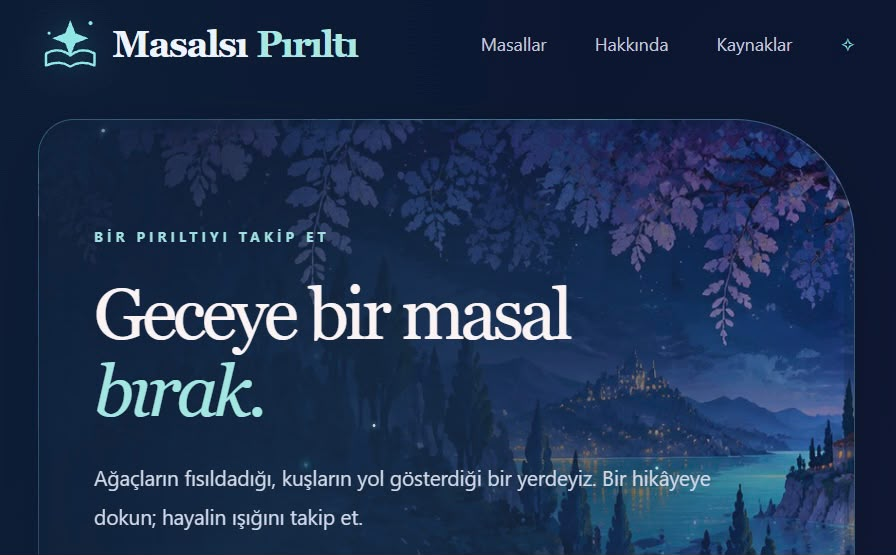
\includegraphics[width=0.9\textwidth]{ekran-masaustu.png}
%   \caption{Sayfanın bilgisayar görünümü}
% \end{figure}

\clearpage
\section{Gerçekleştirme}
% ====================================================================
\aciklama{Sayfanın nasıl çalıştığını kendi cümlelerinizle anlatın. Kodu sunumda
açıklayabilmelisiniz; burada da mantığını yazın. Kodun tamamını değil, önemli
bölümlerini kısa örneklerle gösterin.}

\subsection{HTML Yapısı}
Sayfa; logo ve menünün bulunduğu üst alan, giriş bölümü,
masal kartları, okuma penceresi ve alt alandan oluşuyor.
Üst alan için header, gezinme bağlantıları için nav,
bölümler için section ve alt alan için footer etiketleri
kullanıldı. Başlıklar h1 ve h2, açıklamalar p etiketleriyle
oluşturuldu. Masallar dialog etiketiyle açılan bir
pencerede okunuyor. İşlem düğmeleri için button,
arama kutusu için input kullanıldı

\subsection{İçsel CSS}
Renkler CSS değişkenleriyle tanımlandı. Masal kartları
Grid, menü ve butonlar Flexbox ile düzenlendi.
Medya sorgularıyla düzenin ekran genişliğine uyum
sağlaması sağlandı. Işık noktaları CSS animasyonuyla
hareket ettirildi.

\begin{lstlisting}[caption={İçsel CSS örneği}]
body { background: #0b1630;
    color: #e9e8fa;}
\end{lstlisting}

\subsection{İçsel JavaScript}
Masallar JSON biçiminde dosyanın içinde tutuluyor.
render() fonksiyonu arama ve tema seçimine göre kartları
listeliyor. openStory() seçilen masalı okuma penceresinde
açıyor. Butonlara tıklama ve arama kutusuna yazma olayları
addEventListener ile işlevlere bağlanıyor.

\begin{lstlisting}[caption={İçsel JavaScript'ten önemli bir bölüm}]

search.addEventListener('input', render);
\end{lstlisting}

\subsection{Sayfanın Özellikleri}


% ====================================================================
\section{Yapay Zekâ Kullanımı}
% ====================================================================
Kod desteği, arama, filtreleme ve okuma ayarları ile HTML, CSS ve JavaScript'in bazı bölümlerinde yapay zekâ kullanıldı. Masal illüstrasyonlarında da ChatGPT görsel üretiminden yararlanıldı.

\begin{longtable}{@{}P{2.4cm}P{3.4cm}P{4.1cm}P{3.4cm}@{}}
\toprule
\textbf{Araç} & \textbf{Ne için kullandınız?} & \textbf{İstem (prompt) özeti} & \textbf{Sayfada nerede?} \\
\midrule
\endhead
ChatGPT & Kod oluşturma ve açıklama & Sekiz masallı, arama ve okuma ayarları bulunan bir site hazırlama. & Sayfanın genel yapısı, arama, filtreleme ve okuma ekranı. \\
ChatGPT & Görsel üretimi & Mavi, mor ve turkuaz tonlarında masallara uygun illüstrasyonlar oluşturma ve düzenleme. & Ana sayfa arka planı ve masal illüstrasyonları. \\
\bottomrule
\end{longtable}

\subsection{Anladığım ve Kendim Yaptığım Kısımlar}
Masalları ve kaynaklarını seçtim. Sitenin adını, renk
paletini ve görsel atmosferini belirledim. Başlıklar,
kart biçimleri, karakterlerin görünümü ve ışık efektleri
için değişiklikler istedim. Kodun ve illüstrasyonların
oluşturulmasında yapay zekâ desteği aldım.

Yapay zekâ desteğiyle oluşturulan kod üzerinde başlıkları,
açıklamaları ve masal tanıtımlarını düzenledim. Renk,
yazı boyutu ve boşluk değerlerini değiştirerek tasarımı
tercihlerime göre geliştirdim. Değişikliklerin etkisini
önizlemede kontrol ettim.

% ====================================================================
\section{Haftalık Katkılar}
% ====================================================================
\aciklama{Her hafta ders içinde yaptığınız çalışmayı kısaca yazın (2--4 cümle). Hangi
özelliği eklediğinizi ya da neyi düzelttiğinizi belirtin ve ilgili commit mesajını
ya da bağlantısını ``Commit'' satırına yazın. Her satıra ekran görüntüsü ekleyin:
resimleri \texttt{hafta1.png}, \texttt{hafta2.png}, \ldots{} adıyla Overleaf
projesine yükleyin. Aynı haftaya ikinci bir görsel eklemek için
\texttt{hafta1b.png} gibi bir dosya yükleyin; kendiliğinden görünür.
Her haftanın altındaki kutulardan o hafta için geçerli olanı $\boxtimes$ ile
işaretleyin: dersin kendisinde katılım gösterdiyseniz ``Ders içinde katılım
sergiledim'', o haftayı sonradan tamamladıysanız ``Telafi yaptım''. Telafi
yaptıysanız yapılan çalışmanın metninde bunu açıkça belirtin.}

\begin{longtable}{@{}>{\raggedright\arraybackslash}p{1.7cm}%
                    >{\raggedright\arraybackslash}p{6.4cm}%
                    >{\centering\arraybackslash}p{6cm}@{}}
\toprule
\rowcolor{ana}\textcolor{white}{\textbf{Hafta}} & \textcolor{white}{\textbf{Yapılan çalışma}} & \textcolor{white}{\textbf{Görsel}} \\
\midrule
\endfirsthead
\toprule
\rowcolor{ana}\textcolor{white}{\textbf{Hafta}} & \textcolor{white}{\textbf{Yapılan çalışma}} & \textcolor{white}{\textbf{Görsel}} \\
\midrule
\endhead
\bottomrule
\endfoot

\textbf{1. hafta}\newline [tarih] &
[Bu hafta yaptığınız çalışma.]\newline \textbf{Commit:} [WorldWideWeb projesini anlatan bir sayfa hazırladım. İçeriği HTML’de başlık, paragraf ve bağlantılarla düzenledim. CSS ile yazı tipini, arka planı ve bağlantı renklerini belirledim.]\katilimkutulari &
\haftagorsel{hafta1.png}\haftaek{hafta1b.png} \\
\midrule
\textbf{2. hafta}\newline [tarih] &
[Bu hafta yaptığınız çalışma.]\newline \textbf{Commit:} [Filmin renk paletini, simetrisini ve tipografisini anlatan bir web sayfası hazırladım. İçeriği ana ve alt başlıklarla ayırdım. Filmin görsel dünyasına uygun olarak mor arka plan ve pembe alt başlıklar kullandım.]\katilimkutulari &
\haftagorsel{hafta2.png}\haftaek{hafta2b.png} \\
\midrule
\textbf{3. hafta}\newline [tarih] &
[Bu hafta yaptığınız çalışma.]\newline \textbf{Commit:} [Sayfaya “Günün Mesajı” adlı bir düğme ekledim. Düğmeye tıklandığında JavaScript ile boş paragrafın içeriğini güncelleyerek “Bugün güzel bir gün!” mesajını gösterdim.]\katilimkutulari &
\haftagorsel{hafta3.png}\haftaek{hafta3b.png} \\
\midrule
\textbf{4. hafta}\newline [tarih] &
[Bu hafta yaptığınız çalışma.]\newline \textbf{Commit:} [İlk uygulamada, tıklanınca renkleri açılan dört kartlı bir eşleştirme oyunu hazırladım. JavaScript ile aynı renkteki kartların gizlenmesini, farklı renkteki kartların ise tekrar griye dönmesini sağladım.]\katilimkutulari &
\haftagorsel{hafta4.png}\haftaek{hafta4b.png} \\
\midrule
\textbf{5. hafta}\newline [tarih] &
[Bu hafta yaptığınız çalışma.]\newline \textbf{Commit:} [CodePen’de düğmeye tıklandığında bir kutunun rengini değiştiren örnek üzerinde çalıştım. JavaScript’te if/else koşuluyla kutunun renginin gri ve sarı arasında nasıl değiştiğini inceledim.]\katilimkutulari &
\haftagorsel{hafta5.png}\haftaek{hafta5b.png} \\
\midrule
\textbf{6. hafta}\newline [tarih] &
[Bu hafta yaptığınız çalışma.]\newline \textbf{Commit:} [CodePen’de “Renk Değiştir” düğmesine tıklanınca bir kutunun arka plan rengini değiştiren örnek üzerinde çalıştım. JavaScript’te if/else kullanarak kutu griyse sarıya, sarıysa griye dönmesini sağlayan koşulu inceledim.]\katilimkutulari &
\haftagorsel{hafta6.png}\haftaek{hafta6b.png} \\
\midrule
\textbf{7. hafta}\newline [tarih] &
[Bu hafta yaptığınız çalışma.]\newline \textbf{Commit:} [mesaj veya bağlantı]\katilimkutulari &
\haftagorsel{hafta7.png}\haftaek{hafta7b.png} \\
\midrule
\textbf{8. hafta}\newline [tarih] &
[Bu hafta yaptığınız çalışma.]\newline \textbf{Commit:} [mesaj veya bağlantı]\katilimkutulari &
\haftagorsel{hafta8.png}\haftaek{hafta8b.png} \\
\end{longtable}

% ====================================================================
\section{Test ve Değerlendirme}
% ====================================================================
\aciklama{Sayfayı hangi tarayıcı ve cihazlarda denediniz? Çalışmayan bir özellik
olduysa dürüstçe yazın ve nedenini açıklayın.}

\begin{center}
\rowcolors{2}{acik}{white}
\begin{tabular}{@{}P{6cm}P{3.4cm}P{3.4cm}@{}}
\toprule
\rowcolor{ana}\textcolor{white}{\textbf{Özellik}} & \textcolor{white}{\textbf{Bilgisayar}} & \textcolor{white}{\textbf{Telefon}} \\
\midrule
\relax Masal arama ve rastgele masal seçimi & Çalışıyor & Çalışıyor \\
\relax Masal okuma ekranının açılması & Çalışıyor & Çalışıyor \\
\relax Yazı boyutu değiştirme ve gece modu & Çalışıyor & Çalışıyor \\
\bottomrule
\end{tabular}
\end{center}

\textbf{Denenen tarayıcılar:} [Chrome, Firefox, Edge, Safari vb.]

% ====================================================================
\section{Sunum Videosu}
% ====================================================================
\begin{center}
\begin{tabular}{@{}ll@{}}
\textbf{Video süresi:} & [dakika:saniye] \quad \aciklama{12--18 dakika olmalıdır} \\
\textbf{Görünürlük:} & [Listelenmemiş / Herkese açık] \\
\textbf{Bağlantı:} & \youtubelink \\
\end{tabular}
\end{center}

\subsection{Video Kontrol Listesi}
\aciklama{Teslimden önce hepsini kontrol edin ve kutuları $\boxtimes$ ile işaretleyin.}
\begin{itemize}
  \item[] $\boxtimes$ Süre 12--18 dakika aralığında.
  \item[] $\boxtimes$ Sunum boyunca kameram açık, yüzüm görünüyor.
  \item[] $\boxtimes$ Görünürlük \textbf{Listelenmemiş} ya da Herkese açık; \textbf{Özel} değil.
  \item[] $\boxtimes$ Bağlantıyı gizli pencerede açtım, video oynuyor.
  \item[] $\boxtimes$ YouTube videoyu işlemeyi bitirdi.
  \item[] $\boxtimes$ Videoyu baştan sona izledim; ses ve kamera tüm sunumda var.
  \item[] $\boxtimes$ Kapaktaki bağlantı ile bu bölümdeki bağlantı aynı.
\end{itemize}

% ====================================================================
\section{Sonuç ve Kendi Değerlendirmem}
% ====================================================================
\aciklama{Masalsı Pırıltı projesi sayesinde bir web sayfasını tasarlamayı ve etkileşimli hâle getirmeyi öğrendim. En çok zorlandığım nokta, sayfanın bazı özelliklerinin telefonda bilgisayardaki gibi çalışmamasıydı. Sorunun nerede ortaya çıktığını anlamak için bu özellikleri iki cihazda ayrı ayrı denedim. Gerekli düzenlemeleri yaptıktan sonra sayfayı yeniden kontrol ettim. Bu süreçte, bir sorunla karşılaştığımda adım adım ilerlemenin çözüm bulmayı kolaylaştırdığını fark ettim. Benzer bir proje yaparsam mobil kontrolleri sona bırakmayıp her yeni özelliği eklediğimde test ederim.}

% ====================================================================
\section{Kaynakça}
% ====================================================================
\aciklama{Masal metinleri için yararlandığınız kitap ve sitelerle, teknik kaynakları
(MDN vb.) ve kullandığınız görsel kaynaklarını yazın. Masalları kendi
cümlelerinizle yazmanız gerekir; kaynaklar yalnızca yararlandığınız yerleri
gösterir.}

\begin{thebibliography}{9}
\raggedright

\bibitem{k1}
Türkiye Kültür Portalı.
\emph{Kurnaz Kurt Masalı}.
\url{https://www.kulturportali.gov.tr/portal/kurnazkurtmasali}

\bibitem{k2}
Masal.org.
\emph{Sihirli Tavşan}.
\url{https://www.masal.org/sihirli-tavsan/}

\bibitem{k3}
Masaloku.net.
\emph{Altın Saçlı Kız Masalı}.
\url{https://www.masaloku.net/altin-sacli-kiz-masali/}

\bibitem{k4}
Masal.org.
\emph{Limon Kız}.
\url{https://www.masal.org/limon-kiz/}

\bibitem{k5}

\emph{Akıllı Ormancı Masalı}.
\url{https://masal6.com/masal/akilli-ormanci-masalini-oku/}

\bibitem{k6}
Muzip Masal Cini.
\emph{Altın Bülbül Türk Masalı}.
\url{https://muzipmasalcini.com/altin-bulbul-turk-masali/}

\bibitem{k7}
Masal-oku.tr.
\emph{Zümrüdüanka Kuşu Masalı}.
\url{https://masal-oku.tr/zumruduanka-kusu-masali/}

\bibitem{k8}
Masaloku.net.
\emph{Gülen Ayva Ağlayan Nar}.
\url{https://www.masaloku.net/gulen-ayva-aglayan-nar/}

\end{thebibliography}

% ====================================================================
\appendix
\section{Teslim Kontrol Listesi}
% ====================================================================
\aciklama{Teslim etmeden önce işaretleyin. Bu sayfayı teslim edilen PDF'te bırakabilirsiniz.}
\begin{itemize}
  \item[] $\boxtimes$ MEBİS'e \textbf{yalnızca bu raporun PDF'ini} yükleyeceğim. ZIP ve HTML dosyası yüklemeyeceğim.
  \item[] $\boxtimes$ PDF dosya adı \texttt{OgrenciNo\_AdSoyad\_vize.pdf} biçiminde.
  \item[] $\boxtimes$ Kapaktaki GitHub ve YouTube bağlantıları doğru; PDF'te tıklayıp denedim.
  \item[] $\boxtimes$ GitHub deposunda web sayfası (tek \texttt{.html}), rapor PDF'i, \texttt{.tex} kaynakları ve \texttt{README.md} var.
  \item[] $\boxtimes$ GitHub deposu \textbf{herkese açık} ya da öğretim üyesine erişim verdim.
  \item[] $\boxtimes$ Çalışmamın son hâli teslim saatinden \textbf{önce} depoya gönderildi.
  \item[] $\boxtimes$ Sayfa içsel CSS ve içsel JavaScript kullanıyor, harici dosya gerektirmiyor.
  \item[] $\boxtimes$ Hazır taslak kullanmadım; yapay zekâ kullandıysam Bölüm 5'i doldurdum.
  \item[] $\boxtimes$ Çalışmanın mantığını sunumda anlatabilirim.
\end{itemize}

\end{document}